\documentclass[a4paper, 11pt]{article}
\usepackage{comment} % enables the use of multi-line comments (\ifx \fi)
\usepackage{lipsum} %This package just generates Lorem Ipsum filler text.
\usepackage{fullpage} % changes the margin
\usepackage{graphicx}

\begin{document}
%Header-Make sure you update this information!!!!
\noindent
\large\textbf{Problem Set 1} \hfill \textbf{Jacob Grunwald} \\
\normalsize CSCI 3753 \hfill

\begin{enumerate}
  \item What are the three high level features that are provided by an Operating System? (describe each)
  \begin{enumerate}
    \item Operating systems provide abstraction from the hardware which allows applications to be generalized onto any machince with a standard operating system like Windows or Linux distros.
    \item Operating systems also provide resource arbitration so that multiple applications can use the same resources like the CPU or memory.
    \item Finally, operating systems provide protection from the user and other applications by preventing access to certain memory locations to applications.
  \end{enumerate}
  \item Why does an Operating System need protection from user code?
  \begin{enumerate}
    \item An operating system needs protection from the user so that the user cannot monopolize the system resources or overwrite aspects of the operating system. If the user were to monopolize resources, then all other processes that are attempting to run would starve.
  \end{enumerate}
  \item What are the four major components of an Operating System? (describe each)
  \begin{enumerate}
    \item The scheduler manages when applications will get access to the CPU and provides time slicing information. This allows for multiple applications to run simultaneously.
    \item The memory manager assigns and keeps track of memory. When an application is run, the memory manager translates the virtual address the application is using into a physical location in memmory.
    \item The file system provides the user with a uniform, logical view of information storage. It abstracts the physical properties of its storage devices to a logical storage unit, a file.
    \item Device management takes care of input and output devices and basically everything else connected to the computer. It keeps track of what is connected and the associated drivers.
  \end{enumerate}
  \item How does a user application access system code within the Operating System? (list the steps, describe how CPU knows what code is running)
  \begin{enumerate}
    \item A user application accesses system code by throwing a system interrupt or trap. This accesses the nested interrupt vector table which the OS uses to know what system code is associated with what function the OS needs to perform. When the flag is thrown, the system enters kernal mode then executes its operation. Once complete it resets the mode bit to 0 indicating it is again in user mode and returns control to the user application.
  \end{enumerate}
  \item How are parameters passed to and results returned from a System Call? (describe possible mechanisms)
  \begin{enumerate}
    \item Parameters are passed to a system call when the user application makes the call. The OS accesses the memory requested by the process by looking at the memory location designated by the process. It then returns what it finds or whatever is required by putting it in the memory location designated by the process.
  \end{enumerate}
  \item What are the steps taken to start up a computer?
  \begin{enumerate}
    \item On computer startup, first, the primary bootloader is run from ROM. This typically looks for the location of the secondary bootloader which is on the primary boot device. The secondary bootloader then loads the kernal into RAM which allows it to run.
  \end{enumerate}
  \item What is a Virtual Machine and how does it differ from a physical machine?
  \begin{enumerate}
    \item A virtual machine is run on top of the host operating system and emulates the hardware the guest OS needs. This is different from a physical machine in that the physical machine will take advantage of all of the physical hardware rather than some, but not all.
  \end{enumerate}
  \item Describe the differences between multi-programming and multi-tasking.
  \begin{enumerate}
    \item Multi-programming increases CPU utilization by organizing jobs so that the CPU always has one to execute. With multi-tasking the CPU executes multiple jobs by switching among them, but switches occur so frequently that the users can interact with each program while it is running. This translates to multi-programming being sequential and multi-tasking being concurrent.
  \end{enumerate}
  \item What is a context switch? (describe the mechanism, the reasons for a switch, and what is switched)
  \begin{enumerate}
    \item During a context switch the CPU first needs to save the current state of an application, then load the state of the new application. The CPU does this to support multitasking, and when it occurs, the CPU swaps the application it is running.
  \end{enumerate}
  \item Provde a timing chart for the processes listed below using multi-programming and another using multi-tasking.

  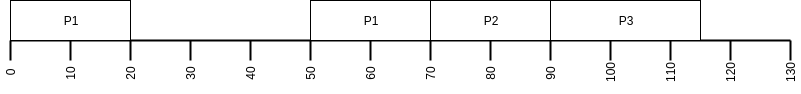
\includegraphics[width=\linewidth]{OS_HW1_1.png}
  \begin{enumerate}
    \item In the case of multiprogramming, process one will run for 20 ticks then block on IO for 30 ticks. In this case I am assuming batch programming rather than the smarter method that would start process two while process one is waiting on IO. Process one will resume at 50 ticks and then complete at 70 ticks. After this proccess two will complete and then process three will complete since they have no IO blocking and there is no time slicing in the mutli-programming.

    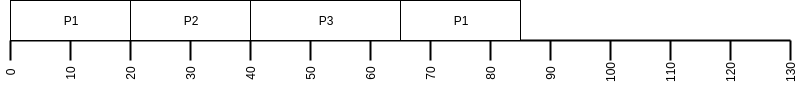
\includegraphics[width=\linewidth]{OS_HW1.png}
    \item In the multitasking case none of the processes take more than 40 ticks to complete and the io blocking from process one ends after process two completes. This makes process three run to completion before 40 ticks pass so process one will resume after 3 completes.
  \end{enumerate}
\end{enumerate}

\end{document}
